
\section{Korektnost a úplnost}\label{section:predicate-resolution-soundness-completeness}

V této sekci dokážeme, že rezoluční metoda je i v predikátové logice korektní a úplná.

\subsection{Věta o korektnosti}

Začneme důkazem korektnosti rezolučního pravidla. Princip je stejný jako u analogického pozorování ve výrokové logice. Důkaz je o trochu techničtější:

\begin{proposition}[Korektnost rezolučního kroku]
Mějme klauzule $C_1$, $C_2$ a nechť $C$ je jejich rezolventou. Platí-li v nějaké struktuře $\A$ klauzule $C_1$ a $C_2$, potom v ní platí i $C$.
\end{proposition}
\begin{proof}
Z definice rezolučního pravidla víme, že klauzule a jejich rezolventu lze vyjádřit jako $C_1=C_1'\sqcup \{A_1,\dots,A_n\}$, $C_2=C_2'\sqcup \{\neg B_1,\dots,\neg B_m\}$, a $C=C_1'\sigma \cup C_2'\sigma$, kde $\sigma$ je
nejobecnější unifikace množiny výrazů $S=\{A_1,\dots,A_n,B_1,\dots,B_m\}$, neboli $S\sigma=\{A_1\sigma\}$.

Protože klauzule $C_1$ a $C_2$ jsou otevřené formule platné v $\A$, platí v $\A$ i jejich instance po substituci $\sigma$ tj. máme $\A\models C_1\sigma$ a $\A\models C_2\sigma$. Víme také, že $C_1\sigma=C_1'\sigma \cup \{A_1\sigma\}$ a podobně $C_2\sigma=C_2'\sigma \cup \{\neg A_1\sigma\}$.

Naším cílem je ukázat, že $\A\models C[e]$ pro libovolné ohodnocení proměnných $e$. Pokud $\A\models A_1\sigma[e]$, potom $\A\not\models\neg A_1\sigma[e]$ a musí být $\A\models C_2'\sigma$. Tedy i $\A\models C$. V opačném případě $\A\not\models A_1\sigma[e]$, musí tedy platit $\A\models C_1'\sigma$, a opět $\A\models C$.
\end{proof}

Znění i důkaz Věty o korektnosti jsou nyní stejné jako ve výrokové logice:

\begin{theorem}[O korektnosti rezoluce]\label{theorem:soundness-of-predicate-resolution}
    Pokud je CNF formule $S$ rezolucí zamítnutelná, potom je nesplnitelná.
\end{theorem}
\begin{proof}
    Víme, že $S\proves_R\square$, vezměme tedy nějaký rezoluční důkaz $\square$ z $S$. Kdyby existoval model $\A\models S$, díky korektnosti rezolučního pravidla bychom mohli dokázat indukcí podle délky důkazu, že i $\A\models\square$, což ale není možné.
\end{proof}


\subsection{Věta o úplnosti}

Větu o úplnosti rezoluce v predikátové logice, totiž že nesplnitelné formule lze zamítnout rezolucí, dokážeme převedením na případ výrokové logiky. Ukážeme, že rezoluční důkaz `na úrovni výrokové logiky' je možné `zvednout' (`lift') na úroveň predikátové logiky.

Klíčem je následující lemma, které zaručuje takové `zvednutí' v jednom rezolučním kroku. Jeho důkaz je poněkud technický. 

\begin{lemma}[Lifting lemma]\label{lemma:lifting-lemma}
Mějme klauzule $C_1$ a $C_2$ s disjunktní množinou proměnných. Jsou-li $C^*_1$ a $C^*_2$ základní instance klauzulí $C_1$ a $C_2$ a je-li $C^*$ je rezolventou $C^*_1$ a $C^*_2$, potom existuje rezolventa $C$ klauzulí $C_1$ a $C_2$ taková, že $C^*$ je základní instancí $C$.
\end{lemma}
\begin{proof}
Nechť $C^*_1=C_1\tau_1$ a $C^*_2=C_2\tau_2$, kde $\tau_1$ a $\tau_2$ jsou základní substituce, které nesdílejí žádnou proměnnou. Najdeme rezolventu $C$ takovou, že $C^*=C\tau_1\tau_2$.

Nechť $C^*$ je rezolventou $C_1^*$ a $C_2^*$ přes literál $P(t_1,\dots,t_k)$. Víme, že klauzule $C_1$ a $C_2$ můžeme vyjádřit jako $C_1=C_1' \sqcup \{A_1,\dots,A_n\}$ a $C_2=C_2' \sqcup \{\neg B_1,\dots,\neg B_m\}$, kde $\{A_1,\dots,A_n\}\tau_1=\{P(t_1,\dots,t_k)\}$ a $\{\neg B_1,\dots,\neg B_m\}\tau_2=\{\neg P(t_1,\dots,t_k)\}$.

To znamená, že $(\tau_1\tau_2)$ unifikuje množinu výrazů $S=\{A_1,\dots,A_n,B_1,\dots,B_m\}$. Nyní vezměme nejobecnější unifikaci $\sigma$ pro $S$ získanou pomocí Unifikačního algoritmu. Jako $C$ zvolme rezolventu $C=C_1'\sigma \cup C_2'\sigma$.

Zbývá ukázat, že $C^*=C\tau_1\tau_2$. Díky vlastnosti `navíc' z Tvrzení \ref{proposition:unification-algorithm} o korektnosti Unifikačního algoritmu víme, že $(\tau_1\tau_2)=\sigma(\tau_1\tau_2)$, což využíváme ve třetí rovnosti z následujícího výpočtu. Ve čtvrté rovnosti využíváme faktu, že $C_1'\tau_1\tau_2=C_1'\tau_1$, a $C_2'\tau_1=C_2'$, což plyne z toho, že jde o základní substituce nesdílející žádnou proměnnou, a že $C_1'\tau_1$ a $C_2'\tau_2$ jsou základní instance:
\begin{align*}
    C\tau_1\tau_2&= (C_1'\sigma \cup C_2'\sigma)\tau_1\tau_2\\
    &=C_1'\sigma\tau_1\tau_2 \cup C_2'\sigma\tau_1\tau_2\\
    &=C_1'\tau_1\tau_2 \cup C_2'\tau_1\tau_2\\
    &=C_1'\tau_1 \cup C_2'\tau_2\\
    &=(C_1\setminus\{A_1,\dots,A_n\})\tau_1\cup (C_2\setminus\{\neg B_1,\dots,\neg B_m\})\tau_2\\
    &=(C_1^*\setminus\{P(t_1,\dots,t_k)\})\cup(C_2^*\setminus \{\neg P(t_1,\dots,t_k)\})=C^*
\end{align*}
\end{proof}

Indukcí podle délky rezolučního důkazu snadno získáme následující důsledek:

\begin{corollary}\label{corollary:lifting}
Mějme CNF formuli $S$ a označme jako $S^*$ množinu všech jejích základních instancí. Pokud $S^*\proves_R C^*$ (`na úrovni výrokové logiky') pro nějakou základní klauzuli $C^*$, potom existuje klauzule $C$ a základní substituce $\sigma$ taková, že $C^*=C\sigma$ a $S\proves_R C$ (`na úrovni predikátové logiky').
\end{corollary}

Nyní už je snadné dokázat úplnost:

\begin{theorem}[O úplnosti rezoluce]\label{theorem:completeness-of-predicate-resolution}
    Je-li CNF formule $S$ nesplnitelná, potom je zamítnutelná rezolucí.
\end{theorem}
\begin{proof}
Označme jako $S^*$ množinu všech základních instancí klauzulí z $S$. Protože je $S$ nesplnitelná, je díky Herbrandově větě (konkrétně Důsledek \ref{corollary:herbrands-theorem-corollary-ground}) nesplnitelná i $S^*$. Z věty o úplnosti \alert{výrokové} rezoluce víme, že $S^*\proves_R\square$ (`na úrovni výrokové logiky'). Z Lifting lemmatu (resp. z Důsledku \ref{corollary:lifting}) dostáváme klauzuli $C$ a základní substituci $\sigma$ takové, že $C\sigma=\square$ a $S\proves_R C$ (`na úrovni predikátové logiky'). Ale protože prázdná klauzule $\square$ je instancí $C$, musí být $C=\square$. Tím jsme našli rezoluční zamítnutí $S\proves_R \square$.
\end{proof}


\section{LI-rezoluce}\label{section:predicate-LI-resolution}

V této sekci připomeneme pojmy \alert{lineárního a linear-input důkazu}, \alert{LI-rezoluci} a její úplnost pro Hornovské formule. Definice i znění vět jsou stejné jako ve výrokové logice (jediným rozdílem je, že v důkazech můžeme používat \alert{varianty} klauzulí z $S$), důkaz lze provést převedením na výrokovou logiku opět pomocí Herbrandovy věty a Lifting lemmatu.

\begin{definition}[Lineární a LI důkaz]
    \alert{Lineární důkaz} (rezolucí) klauzule $C$ z formule $S$ je konečná posloupnost
    $$
    \begin{bmatrix}
        C_0 \\
        B_0
    \end{bmatrix},
    \begin{bmatrix}
        C_1 \\
        B_1
    \end{bmatrix},\dots,
    \begin{bmatrix}
        C_n \\
        B_n
    \end{bmatrix},
    C_{n+1}
    $$
    kde $C_i$ říkáme \alert{centrální} klauzule, $C_0$ je \alert{počáteční}, $C_{n+1}=C$ je \alert{koncová}, $B_i$ jsou \alert{boční} klauzule, a platí:
    \begin{itemize}
        \item $C_0$ je varianta klauzule z $S$, pro $i\leq n$ je $C_{i+1}$ rezolventou $C_i$ a $B_i$,
        \item $B_0$ je varianta klauzule z $S$, pro $i\leq n$ je $B_i$ varianta klauzule z $S$ nebo $B_i=C_j$ pro nějaké $j<i$. 
    \end{itemize}
    \alert{Lineární zamítnutí} $S$ je lineární důkaz $\square$ z $S$.
    
    \alert{LI-důkaz} je lineární důkaz, ve kterém je každá boční klauzule $B_i$ variantou klauzule z $S$. Pokud existuje LI-důkaz, říkáme, že je $C$ \alert{LI-dokazatelná} z $S$, a píšeme $S\proves_{LI}C$. Pokud $S\proves_{LI}\square$, je $S$ \alert{LI-zamítnutelná}.
\end{definition}

V Poznámce \ref{remark:linear-resolution} jsme poznamenali, že `lineární' rezoluce (založená na lineárních důkazech) je úplná. Důkaz byl ponechán jako cvičení. Stejné tvrzení platí i v predikátové rezoluci:

\begin{theorem}[O úplnosti lineární rezoluce]
Klauzule $C$ má lineární důkaz z CNF formule $S$, právě když má rezoluční důkaz z $S$ (tj. $S\proves_R C$).
\end{theorem}
\begin{proof}
Z lineárního důkazu snadno vyrobíme rezoluční strom. Opačná implikace plyne z Poznámky \ref{remark:linear-resolution} a z Lifting lemmatu (jehož použití zachovává linearitu rezolučního důkazu).
\end{proof}

\subsection{Úplnost LI-rezoluce pro Hornovy formule}

Připomeňme terminologii týkající se hornovskosti a programů: \alert{Hornova klauzule} je klauzule obsahující nejvýše jeden pozitivní literál. \alert{Hornova formule} je (konečná, nebo i nekonečná) množina Hornových klauzulí.
\alert{Fakt} je pozitivní jednotková (Hornova) klauzule, \alert{pravidlo} je (Hornova) klauzule s právě jedním pozitivním a alespoň jedním negativním literálem, a \alert{cíl} je neprázdná (Hornova) klauzule bez pozitivního literálu. Pravidlům a faktům říkáme \alert{programové klauzule}.

Stejně jako ve výrokové logice, LI-rezoluce je úplná pro Hornovské formule:

\begin{theorem}[O úplnosti LI-rezoluce pro Hornovy formule]\label{theorem:completeness-of-li-resolution-for-horn-predicate}
Je-li Hornova formule $T$ splnitelná, a $T\cup\{G\}$ je nesplnitelná pro cíl $G$, potom $T\cup\{G\}\proves_{LI}\square$, a to LI-zamítnutím, které začíná cílem $G$.   
\end{theorem}
\begin{proof}
    Plyne z analogické věty ve výrokové logice, z Herbrandovy věty, a z Lifting lemmatu
\end{proof}


\subsection{(draft) Rezoluce v Prologu}\todo

% from slides:
\subsubsection*{Program v Prologu}
    \mdef{Program} (v Prologu) je Hornova formule obsahující pouze \myblue{programové}
    \smallskip
    
    \myblue{klauzule}, tj. \myblue{fakta} nebo \myblue{pravidla}.
    \bigskip
    
    \centerline{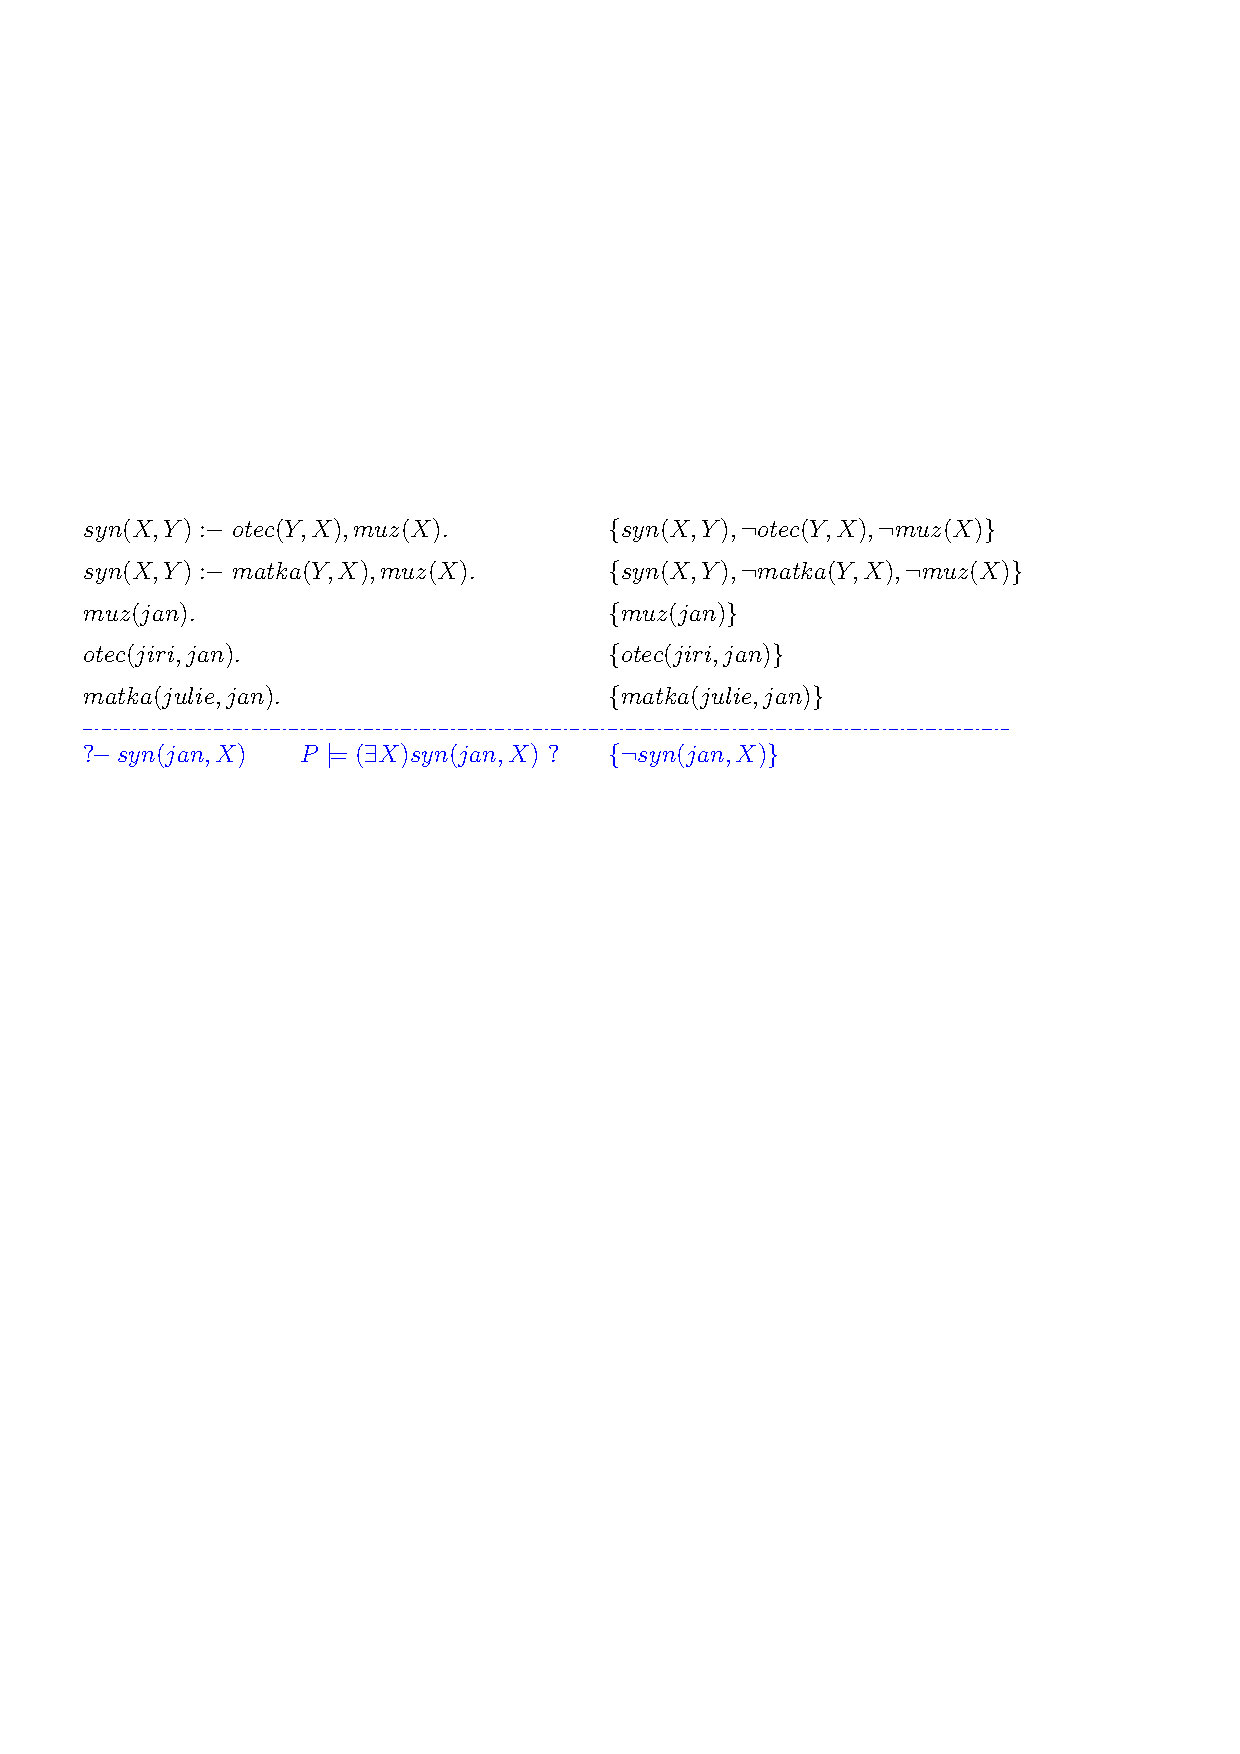
\includegraphics[scale=0.7]{files/rezolucePLprogram}}
    \bigskip
    
    {\it Zajímá nás, zda daný \myblue{existenční dotaz} vyplývá z daného programu.}%, navíc to chceme doložit \myblue{výstupní substitucí}.
    \medskip
    
    {\bf \myblue{Důsledek}}\ \ {\it Pro program $P$ a cíl $G=\{\neg A_1, \dots, \neg A_n\}$ v proměnných $X_1,\dots,X_m$
    
    \vspace{-0mm}
    \begin{enumerate}
    \item[$(1)$] $P \models (\exists X_1)\dots(\exists X_m)(A_1\mand \dots \mand A_n)$, právě když
    \smallskip
    
    \item[$(2)$] $\square$ lze odvodit LI-rezolucí z $P\cup\{G\}$ začínající (variantou) cíle $G$.
    \end{enumerate}}
    
    
    %%%%%%%%%%%%%%%%%%%%%%%%%%%%%%%%%%%%%%%%%%%%%%%%%%%%%%5
    
    \subsubsection*{LI-rezoluce nad programem}
    {\it Je-li odpověď na dotaz kladná, chceme navíc znát výstupní substituci.}
    \medskip
    
    \mdef{Výstupní substituce} $\sigma$ LI-rezoluce $\square$ z $P\cup\{G\}$ začínající $G=\{\neg A_1,\dots,\neg A_n\}$
    \smallskip
    
    je složení \myblue{mgu} v jednotlivých krocích (jen na proměnné v $G$). Platí,
    \vspace{-2mm}
    \mygreen{$$P \models (A_1 \mand \dots \mand A_n)\sigma.$$}
    
    \vspace{-2mm}
    
    \centerline{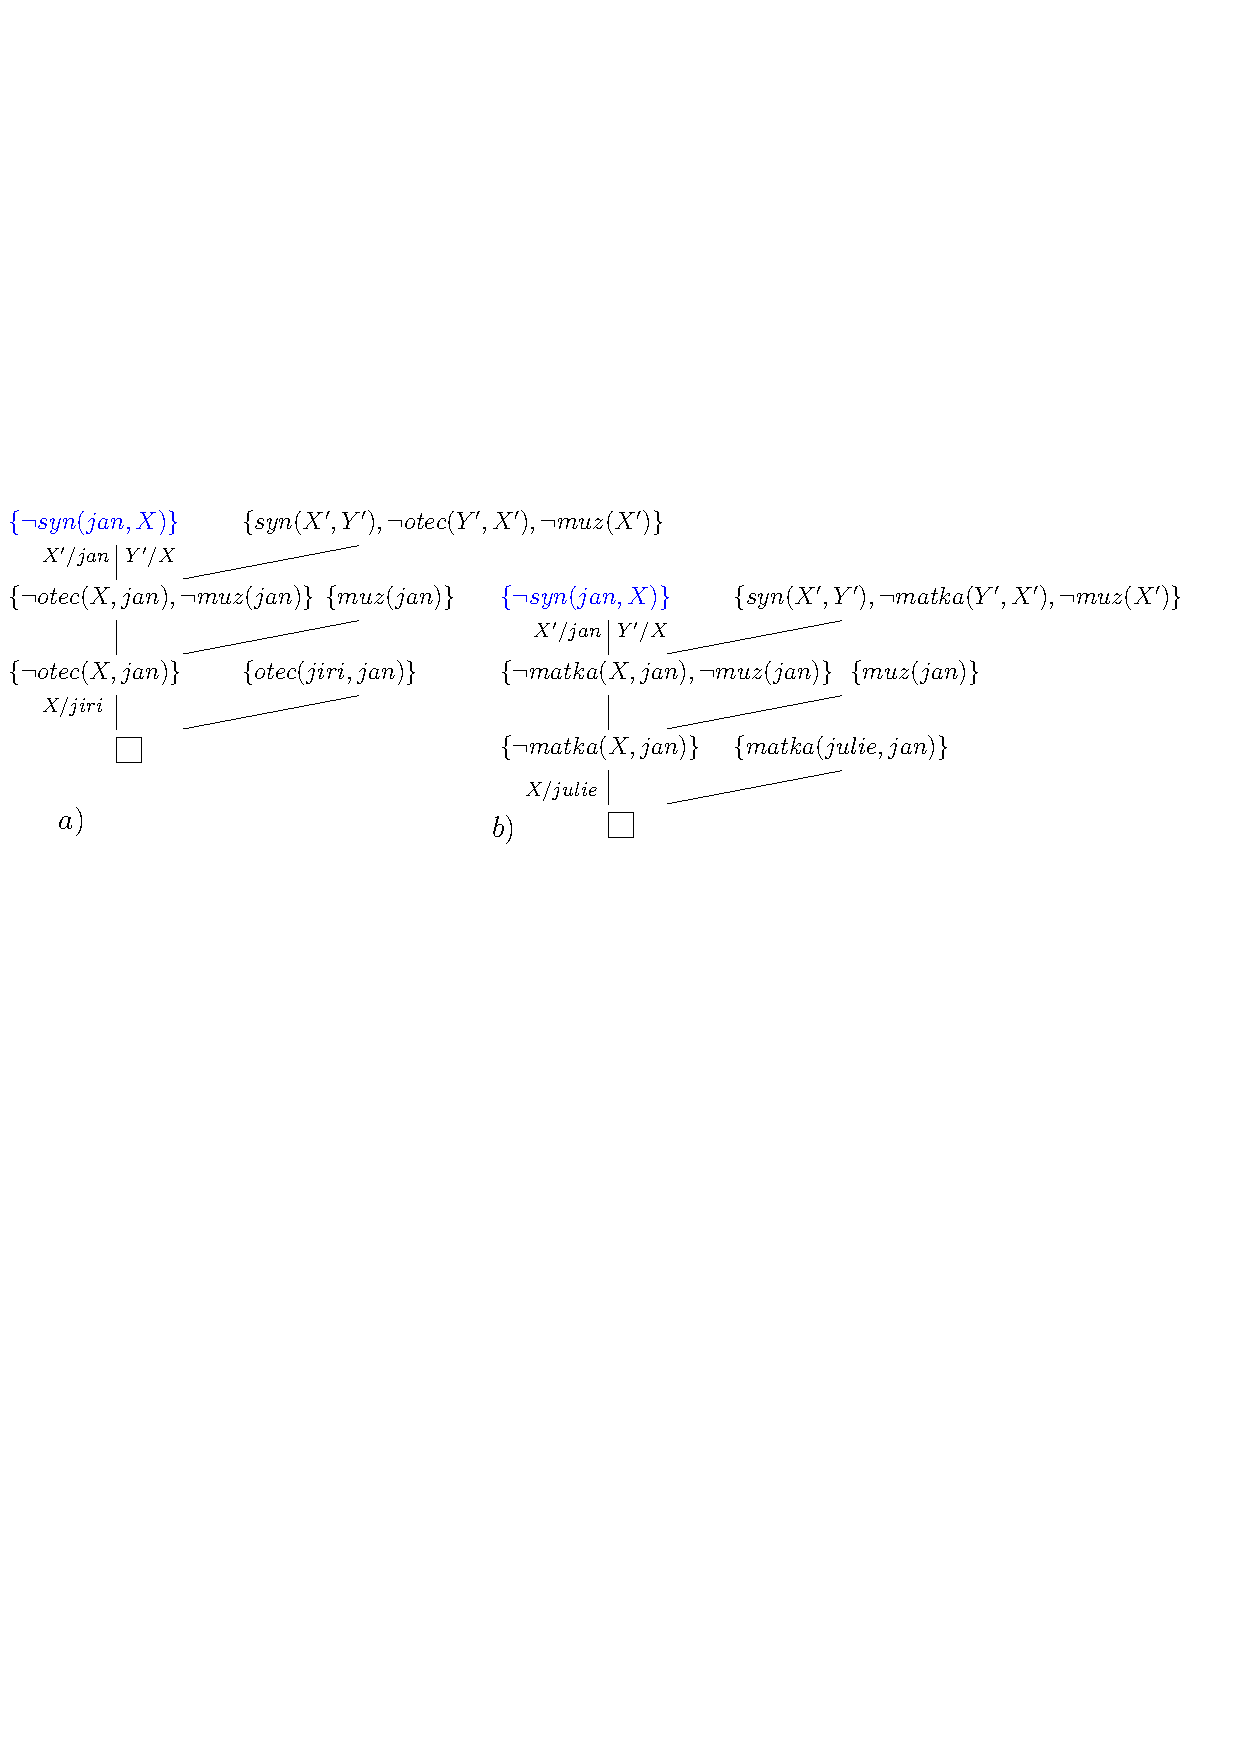
\includegraphics[scale=0.63]{files/rezolucePLprogramLI}}
    \bigskip
    
    Výstupní substituce $a)$ $X=jiri$,\ \ $b)$ $X=julie$.
    
    
% :from slides
